% Generated by scripts/make_explanation_figures.py from experiment_0013 (do not edit by hand).
% Model: COVER
\documentclass[tikz,border=3pt]{standalone}
\usepackage[T1]{fontenc}
\usepackage[utf8]{inputenc}
\usepackage{newtxtext,newtxmath}
\usetikzlibrary{positioning,arrows.meta,calc}

\definecolor{neural}{HTML}{2F6DB5}
\definecolor{neuralbg}{HTML}{E8F0FA}
\definecolor{logic}{HTML}{2E8B57}
\definecolor{logicbg}{HTML}{E6F4EC}
\definecolor{relneg}{HTML}{C0392B}

\tikzset{
  tok/.style={draw=neural!80, fill=white, rounded corners=1.5pt, inner sep=1.6pt, font=\scriptsize,
              minimum height=4mm, anchor=base},
  htok/.style={tok, fill=neural!12},
  stok/.style={tok, draw=black!25, text=black!45},
  aedge/.style={line width=#1, draw=logic},
  cedge/.style={line width=#1, draw=relneg},
  ledge/.style={line width=#1, draw=neural, densely dashed},
  rlab/.style={font=\tiny, fill=white, inner sep=0.6pt},
}
\newcommand{\bars}[4]{%
  \fill[logic]  (#1-0.17,0.05) rectangle ++(0.15,{0.8*#2});
  \fill[relneg] (#1+0.02,0.05) rectangle ++(0.15,{0.8*#3});
  \node[font=\tiny, anchor=north] at (#1-0.095,0.03) {$s$};
  \node[font=\tiny, anchor=north] at (#1+0.095,0.03) {$c$};
  \node[font=\tiny, anchor=north] at (#1,-0.22) {$#2\,/\,#3$};
  \node[font=\tiny, anchor=north, text=black!60] at (#1,-0.47) {$\omega{=}#4$};
}
\newcommand{\sbar}[3]{%
  \fill[logic]  (#1-0.075,0.05) rectangle ++(0.15,{0.8*#2});
  \node[font=\tiny, anchor=north] at (#1,0.03) {$s$};
  \node[font=\tiny, anchor=north] at (#1,-0.22) {$#2$};
  \node[font=\tiny, anchor=north, text=black!60] at (#1,-0.47) {$\omega{=}#3$};
}
\providecommand{\Pcov}{P_{\mathrm{cov}}}
\providecommand{\Pnc}{P_{\neg\mathrm{conf}}}
\providecommand{\E}{\textsc{e}}
\providecommand{\N}{\textsc{n}}
\providecommand{\C}{\textsc{c}}

\begin{document}
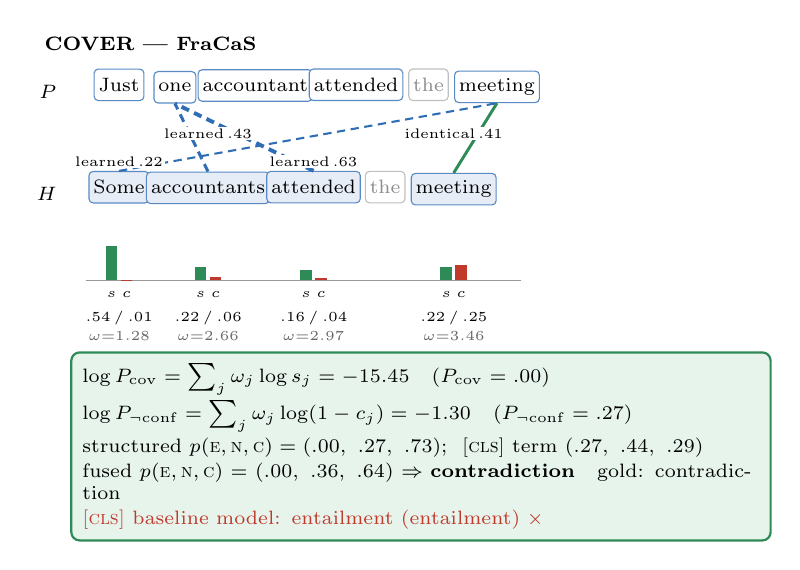
\begin{tikzpicture}
\node[font=\scriptsize\itshape, anchor=east] at (-0.35,2.45) {$P$};
\node[font=\scriptsize\itshape, anchor=east] at (-0.35,1.15) {$H$};
\node[tok] (p1) at (0.32,2.45) {Just};
\node[tok] (p2) at (1.03,2.45) {one};
\node[tok] (p3) at (2.05,2.45) {accountant};
\node[tok] (p4) at (3.33,2.45) {attended};
\node[stok] (pw4) at (4.25,2.45) {the};
\node[tok] (p6) at (5.12,2.45) {meeting};
\node[htok] (h10) at (0.32,1.15) {Some};
\node[htok] (h11) at (1.45,1.15) {accountants};
\node[htok] (h13) at (2.79,1.15) {attended};
\node[stok] (hw3) at (3.70,1.15) {the};
\node[htok] (h15) at (4.57,1.15) {meeting};
\draw[ledge=0.75pt] (h10.north) -- (p6.south);
\draw[ledge=1.09pt] (h11.north) -- (p2.south);
\draw[ledge=1.40pt] (h13.north) -- (p2.south);
\draw[aedge=1.06pt] (h15.north) -- (p6.south);
\node[rlab, anchor=south] at (0.32,1.47) {learned\,.22};
\node[rlab, anchor=south] at (1.45,1.83) {learned\,.43};
\node[rlab, anchor=south] at (2.79,1.47) {learned\,.63};
\node[rlab, anchor=south] at (4.57,1.83) {identical\,.41};
\draw[black!40] (-0.1,0.05) -- (5.42,0.05);
\bars{0.32}{.54}{.01}{1.28}
\bars{1.45}{.22}{.06}{2.66}
\bars{2.79}{.16}{.04}{2.97}
\bars{4.57}{.22}{.25}{3.46}
\node[draw=logic, fill=logicbg, rounded corners=3pt, line width=0.8pt, font=\scriptsize, align=left, anchor=north west, text width=8.60cm, inner sep=4pt] (agg) at (-0.3,-0.85) {%
  $\log\Pcov=\sum_j\omega_j\log s_j=-15.45$\quad($\Pcov=.00$)\\[1pt]$\log\Pnc=\sum_j\omega_j\log(1-c_j)=-1.30$\quad($\Pnc=.27$)\\[1pt]structured $p(\E,\N,\C)=(.00,\ .27,\ .73)$;\ \ \textsc{[cls]} term $(.27,\ .44,\ .29)$\\[1pt]fused $p(\E,\N,\C)=(.00,\ .36,\ .64)$ $\Rightarrow$ \textbf{contradiction}\quad gold: contradiction\\[1pt]\textcolor{relneg}{\textsc{[cls]} baseline model: entailment (entailment) \texttimes}};
\node[font=\scriptsize\bfseries, anchor=south west] at (-0.75,2.85) {COVER --- FraCaS};
\end{tikzpicture}
\end{document}
